\chapter{Deterministic RL-MPC}
\label{chapter:deterministic_RL_MPC}

This chapter aims to construct the RL-MPC framework and examines various implementations to determine their effectiveness. The resulting contollers are evaluated by comparing it with the MPC and RL controllers developed in previous sections. The implementations serve as a means for the reader to understand the construction of the final RL-MPC algorithm, as each subsequent implementation builds upon the previous one. In addition, this chapter will analyze the nominal case in which the parameters of the model and environment are known. 

The smoothness of the value function curve is crucial because, when optimized, it can lead to the generation of numerous local optima, which can disrupt the controller's performance.


\section{Implementation} \label{section:rlmpc implementation}
While there are numerous implementations of RL-MPC, there is limited research focused on maximizing economic benefit specifically for continuous state and action spaces while training RL separately from MPC. As stated in \cite{ellisTutorialReviewEconomic2014} and \cite{amritEconomicOptimizationUsing2011}, an EMPC without a terminal constraint and/or terminal cost function does not provide performance and stability guarantees. Specifically \cite{ellisTutorialReviewEconomic2014} states that a terminal constraint is required to ensure closed-loop performance, while \cite{amritEconomicOptimizationUsing2011} extends this concept by proving that applying a terminal region constraint with an appropriate terminal cost function is required to guarantee closed-loop performance. \cite{amritEconomicOptimizationUsing2011} further claims that the terminal cost function with a terminal region is superior to the terminal constraint because it increases the size of the feasible set of initial conditions and may possibly improve the closed-loop performance. However finding such suitable terminal constraints and cost functions prove to be very difficult. It is the objective of this thesis is to ascertain whether the RL agent is capable of providing this.\\
Furthermore, when considering the RL perspective in these implementations, it is important to note that the learned value function is merely an approximation. Consequently, when this value function is utilised in MPC, it is effectively unrolled and value iterations are executed. This process has the potential to result in an improved policy compared to the original policy that generated the value function.


The integration of RL into MPC will increasingly involve more complex implementations to analyze the impact at each stage. Firstly, initial guesses from the actor will be examined. Subsequently, a terminal constraint will be established by the RL agent. Following this, a terminal constraint region will be defined, also determined by the RL agent. The various value functions as trained by the nominal agent (\autoref{tab:various-vf}) will then be used as the terminal cost function, with and without the terminal region constraint. Lastly, a parallel problem will be presented in order to explore an slightly alternative application of the value function.

\subsection{RL-MPC problem formulations}

\paragraph{Implementation 1}
Implementation 1 is identical to \autoref{eq:mpc_ocp}, but with the inclusion of initial guesses. However, instead of utilising the previous solution to the state and input trajectories as initial guesses, these initial guesses are provided by the RL agent. Two sets of initial guesses will be tested and compared with one another. The solution to the OCP in \autoref{eq:mpc_ocp} at time $k$  can be denoted as:

\begin{equation}\label{eq:sol-mpc-ocp}
	\begin{aligned}
		&\mathbf{x}_{k|k} = [x_{k|k},x_{k_+ 1|k},x_{k + 2|k}, ...,x_{k + N_p|k}]^T \\ 
		&\mathbf{u}_{k|k} = [u_{k|k},u_{k + 1|k}, ...,u_{k + N_p-1|k}]^T \\
	\end{aligned}
\end{equation}

The two sets of initial guesses at the $k$ step is denoted as:

\begin{equation}\label{eq:initial-guess-1}
	\begin{aligned}
		&\tilde{\mathbf{x}}_{k|k} = [\tilde{x}_{k|k},\tilde{x}_{k+1|k},...,\tilde{x}_{k + N_p|k}]^T \\ 
		&\tilde{\mathbf{u}}_{k|k} = [\tilde{u}_{k|k},\tilde{u}_{k + 1|k},...,\tilde{u}_{k + N_p - 1|k}]^T\\ 
	\end{aligned}
\end{equation}

\begin{equation}\label{eq:initial-guess-2}
	\begin{aligned}
		&\hat{\mathbf{x}}_{k|k} = [\hat{x}_{k|k},\hat{x}_{k+1|k},...,\hat{x}_{k + N_p|k}]^T \\ 
		&\hat{\mathbf{u}}_{k|k} = [\hat{u}_{k|k},\hat{u}_{k + 1|k},...,\hat{u}_{k + N_p - 1|k}]^T\\ 
	\end{aligned}
\end{equation}

such that

 \begin{equation}\label{eq:horizon_extension}
 	\begin{aligned}
 		&\tilde{\mathbf{x}}_{k|k} = &[\mathbf{x}_{k|k-1},f(x_{k-1 + N_p|k-1}, \pi(x_{k-1 + N_p|k-1}), d_{k+Np|k},p)]^T\\ 
 		&\tilde{\mathbf{u}}_{k|k} = &[\mathbf{u}_{k|k-1},\pi(x_{k-1 + N_p|k-1})]^T\\
 	\end{aligned}
 \end{equation}

\begin{equation}\label{eq:actor_roll_out}
	\begin{aligned}
		&\hat{\mathbf{x}}^{k_1} = [x_{k_1},f(x_{k_1},\pi(x_{k_1}),d_{k_1},p),..., f(x_{k_1 + N_p-1}, \pi(x_{k_1 + N_p-1}), d_{k_1 + Np-1},p)]^T \\ 
		&\hat{\mathbf{u}}^{k_1} = [\pi(x_{k_1},\pi(x_{k_1+1}),...,\pi(x_{k_1+Np-1})]^T \\ 
	\end{aligned}
	\end{equation}


%\begin{equation}\label{eq:initial-guess-1}
%	\begin{aligned}
%		&\tilde{\mathbf{x}}_{k+1|k+1} = [x_{k + 1|k+1},...,x_{k + N_p}|k+1, f(x_{k + N_p|k+1}, \pi(x_{k + N_p|k+1}), d_{k_0 + Np},p)]^T \\ 
%		&\tilde{\mathbf{u}}^{k_1} = [u_{k_0 + 1},...,u_{k_0 + N_p - 1}, \pi(x_{k_0 + N_p})]^T \\ 
%	\end{aligned}
%\end{equation}
%
%\begin{equation}\label{eq:initial-guess-2}
%	\begin{aligned}
%	&\hat{\mathbf{x}}^{k_1} = [x_{k_1},f(x_{k_1},\pi(x_{k_1}),d_{k_1},p),..., f(x_{k_1 + N_p-1}, \pi(x_{k_1 + N_p-1}), d_{k_1 + Np-1},p)]^T \\ 
%	&\hat{\mathbf{u}}^{k_1} = [\pi(x_{k_1},\pi(x_{k_1+1}),...,\pi(x_{k_1+Np-1})]^T \\ 
%\end{aligned}
%\end{equation}

The first initial guess (\autoref{eq:initial-guess-1}) takes the previous time steps solution, shifts it and uses the policy $\pi(\cdot)$, as provided by the actor, to calculate the optimal action and resulting state to take at the last time step. Essentially the actor is unrolled once from the last time step of the previous solution to \autoref{eq:mpc_ocp}. The second initial guess,\autoref{eq:initial-guess-2}, involves unrolling the actor $Np$ steps from the current state, and using the resulting actions and states as initial guesses. 

\paragraph{Implementation 2}
The second implementation incorporates a terminal constraint. The asymptotic average performance of the EMPC can be guaranteed to be no worse than the performance of a optimal reference trajectory under certain assumptions. From \cite{amritEconomicOptimizationUsing2011}, these assumptions are:

\hspace{1cm} \textbf{Assumption 1} (Properties of constraint sets) The set $\mathbb{Z}$ is compact, where $\mathbb{Z} \subseteq \mathbb{X} \times \mathbb{U}$

\hspace{1cm} \textbf{Assumption 2}  (Continuity of cost and system) The functions $l(\cdot), f(\cdot)$ are continuous on $\mathbb{Z}$. The terminal cost function $V_f(\cdot)$ is continuous on $\mathbb{X}_f$ 

\hspace{1cm} \textbf{Assumption 3} (Stability assumption) There exist a compact terminal region $\mathbb{X}_f \subseteq \mathbb{X}$, containing the point $x_s$ in its interior, and control law $\kappa_f : \mathbb{X}_f \rightarrow \mathbb{U}$, such that the following holds 
\begin{equation}\label{eq:assumption_3}
	V_f(f(x,\kappa_f(x))) \leq V_f(x) - l(x,\kappa_f(x)) + l(x_s,u_s) \quad \forall x \in \mathbb{X}_f
\end{equation}

Assumptions 1 and 2 holds since all states and inputs are bounded and the stage cost, as defined in \autoref{eq:mpc_stage_cost} is continuous. For this implementation, $V_f(\cdot) \equiv 0$, therefore, assumption 3 clearly holds since $x,\kappa_f(x)$ is constrained to $x_s,u_s$.
 \cite{risbeckEconomicModelPredictive2020}, \cite{amritEconomicOptimizationUsing2011} proves that to ensure this for a time-varying system a reference trajectory ($\tilde{\mathbf{x}},\tilde{\mathbf{u}}$) that serves as a bases for a meaningful economic performance for the system must be provided. The terminal constraint should be imposed to keep the system close to this reference trajectory. Since the RL policy can be used as the optimal reference policy, it can be guaranteed that the resulting policy will be at least as good as the RL policy. In order to keep the EMPC close to RL's reference trajectory, initial guesses as given in \autoref{eq:initial-guess-1} with a terminal constraint equal to the last initial guess such that:

\begin{equation}\label{eq:terminal-constraint-ocp}
	\begin{aligned}
		& x^{k_0}_{Np} = \mathbf{e}_{Np}^T \tilde{\mathbf{x}}^{k_0}\\
		& u^{k_0}_{Np-1} = \mathbf{e}_{Np-1}^T\tilde{\mathbf{u}}^{k_0}\\
	\end{aligned}
\end{equation}

where $\mathbf{e}_{Np+1}$ and $\mathbf{e}_{Np}$ represents the $i$th standard basis vector in $\mathbb{R}^{Np+1}$ and $\mathbb{R}^{Np}$ respectively. i.e., $e_i$ provides a selection vector to extract the last state and input from the initial guess, to be used as a terminal constraint. Both the last control input and the state must be constrained since the current control action depends on the previous control action (\autoref{eq:constraint-delta-u}).

\paragraph{Implementation 3}
Implementation 3 builds upon implementation 2, in that instead of providing a terminal constraint, a terminal region as provided by the actor will be used. The terminal region is defined as:

\begin{equation}\label{eq:terminal-region}
	\begin{aligned}
		& (1-\delta_T)\mathbf{e}_{Np}^T \tilde{\mathbf{x}}^{k_0} \leq x^{k_0}_{Np} \leq (1+\delta_T)\mathbf{e}_{Np}^T \tilde{\mathbf{x}}^{k_0}\\
		&(1-\delta_T)\mathbf{e}_{Np-1}^T\tilde{\mathbf{u}}^{k_0} \leq u^{k_0}_{Np-1} \leq (1+\delta_T) \mathbf{e}_{Np-1}^T\tilde{\mathbf{u}}^{k_0}\\
	\end{aligned}
\end{equation}

\cite{amritEconomicOptimizationUsing2011} suggests that this has the same performance guarantees as Implementation 2 under the same assumptions. However introducing a terminal region for the terminal state makes it difficult to meet assumption 3 as shown in \autoref{eq:assumption_3}. However, \cite{amritEconomicOptimizationUsing2011} suggest that providing a terminal region may be more beneficial than a terminal constraint. Finally, a terminal constraint and initial guesses will also be provided by \autoref{eq:initial-guess-2} to investigate performance. However, since the action of unrolling from the current state does not result in following a fixed trajectory, no performance guarantee can be made.

\paragraph{Implementation 4}
Implementation 4 consists of only including the value function as learned in \autoref{section:trained-vf}, and initial guesses as given in \autoref{eq:initial-guess-1}. This implementation examines the effect of the value function on the performance of the resulting controller. The value function can be incorporated into \autoref{eq:mpc_ocp} by defining a cost function:

\begin{equation}\label{eq:cost-function}
		\min_{u(k),x(k)}  \sum_{k = k_0}^{k_0 + N_p - 1}{l(u(k), y(k))} - \tilde{V}(s'(k_0 + N_p))
\end{equation}

where $\tilde{V}$ represents the learned value function and $s'(k_0+N_p)$ is the normalization of $s(k_0+N_p)$. For $\tilde{V}^1$,$\tilde{V}^2$,$\tilde{V}^3$, the unnormalized input is \autoref{eq:obs-tuple-1}, where as in $\tilde{V}^4$, this is $(y_{k_0+N_p},k_0+N_p)$ as discussed in \autoref{section:trained-vf}. Normalization of the state observation is performed with \autoref{eq:state-normalization}. This implementation aims to evaluate the impact of different neural network architectures, including a deep neural network ($\tilde{V}^1$), a smaller deep neural network ($\tilde{V}^2$), a shallow neural network ($\tilde{V}^3$), and a deep neural network trained to learn the value function on only two system states. This can be considered a naive implementation of RL-MPC, and would essentially equate to the rolling out the value function. According to approximate dynamic programming as stated in \cite{bertsekasLessonsAlphaZeroOptimal}, this policy could be better than the policy that generated the value function. The performance is heavily dependent on the quality of the value function. If the approximate value function is inaccurate and the errors are significant and systematic then unrolling this value function could lead to a worse policy. This implementation may be conceptually viewed as either unrolling the value function, or providing the MPC knowledge of the future, essentially extending its prediction horizon. 
Note that the value function is maximized by minimizing the negative of it, since the learned value function represents total return and not cost.

\paragraph{Implementation 5}
Implementation 5 essentially combines Implementation 3 and Implementation 4. \cite{amritEconomicOptimizationUsing2011} states that finding an appropriate terminal cost function and corresponding terminal region proves to be non-trivial in order to satisfy assumption 3. This implementation is also claimed to be superior to the terminal constraint of implementation 2 (\cite{amritEconomicOptimizationUsing2011}) under necessary conditions. Therefore the resulting RL-MPC OCP is defined as:

\begin{subequations} \label{eq:rl-mpc-ocp}
	\begin{align}
		\min_{u(k),x(k)} & \sum_{k = k_0}^{k_0 + N_p-1} {l(u(k), y(k))} - \tilde{V}(s(k_0+N_p)) \\
		\text{s.t.} \quad & x(k+1) = f(x(k), u(k), d(k), p),  \label{eq:rl-mpc-dynamics-constraint} \\
		& y(k) = g(x(k+1), p), \label{eq:rl-mpc-output-constraint} \\
		& -\delta u \leq u(k) - u(k-1) \leq \delta u, \label{eq:rl-mpc-delta-u} \\
		& u_{\min} \leq u(k) \leq u_{\max}, \label{eq:rl-mpc-u-limits}\\
		& x(k_0) = x_{k_0}. \label{eq:rl-pmc-initial} \\
		&\tilde{\mathbf{x}}^{k_0} = [x_{k_{-1} + 1},...,x_{k_{-1} + N_p}, f(x_{k_{-1} + N_p}, \pi(x_{k_{-1} + N_p}), d_{k_{-1} + Np},p)]^T \\ 
		&\tilde{\mathbf{u}}^{k_{0}} = [u_{k_{-1} + 1},...,u_{k_{-1} + N_p - 1}, \pi(x_{k_{-1} + N_p})]^T \\ 
		& (1-\delta_T)\mathbf{e}_{Np}^T \tilde{\mathbf{x}}^{k_0} \leq x^{k_0}_{Np} \leq (1+\delta_T)\mathbf{e}_{Np}^T \tilde{\mathbf{x}}^{k_0}\\
		&(1-\delta_T)\mathbf{e}_{Np-1}^T\tilde{\mathbf{u}}^{k_0} \leq u^{k_0}_{Np-1} \leq (1+\delta_T) \mathbf{e}_{Np-1}^T\tilde{\mathbf{u}}^{k_0}\\
	\end{align}
\end{subequations}

This implementation was investigated to determine whether RL might provide both an adequate terminal region and cost function to improve the MPC's performance.


\paragraph{Implementation 6}
Implementation 6 serves an alternative method of incorporating the value function. This implementation involves solving implementation 3 however with \autoref{eq:initial-guess-1} and \autoref{eq:initial-guess-2} separately. Once solved, the terminal state of the two solution trajectories are compared by evaluating them with the value function. The solution trajectory with the terminal state that yields the most favourable outcome (as given from the value function) is selected as the final solution and the first control input of this solution is taken. It essentially selects the best policy. Although only 2 policies are compared, this method may warrant further research whereby multiple generated policies could be compared. The policies generated could originate from multiple RL agents, each providing their initial estimations along with corresponding terminal constraints. Although each problem could be solved in parallel to speed up computational speed, it was implemented sequentially in this thesis.



\subsection{Initial RL and MPC performance}
A review of the RL and MPC policies will be evaluated for the nominal conditions.

\begin{figure}[H]
	\centering
	\begin{subfigure}[b]{0.49\textwidth}
		\centering
		\includegraphics[width=\textwidth]{figures/mpc_vs_rl_perf.eps}
		\caption{MPC vs RL Performance}
		\label{fig:mps-vs-rl-perf}
	\end{subfigure}
	\hfill
	\begin{subfigure}[b]{0.49\textwidth}
		\centering
		\includegraphics[width=\textwidth]{figures/mpc_vs_rl_time.eps}
		\caption{MPC vs RL compute time}
		\label{fig:mpc-vs-rl-time}
	\end{subfigure}
	\caption{MPC vs RL}
	\label{fig:mpc-vs-rl}
\end{figure}

\autoref{fig:mpc-vs-rl} demonstrated the performance of the MPC and RL agent in the nominal setting. Although MPC does perform better for all prediction horizons (except 1 hour) as shown in \autoref{fig:mps-vs-rl-perf}, it does not imply that this is the best RL policy obtainable. A more extensive hyper parameter tuning may have to be forgone in order to achieve a policy that outperforms MPC. However the RL agent is clearly competitive and as seen in \autoref{fig:mpc-vs-rl-time}, can compute actions significantly faster. It is evident that the RL agent can be utilized to generate a reference trajectory for MPC with minimal increase in computational time. The performance of the resulting RL-MPC and its potential superiority will be analyzed in following sections and compared to the baseline performances, as depicted in \autoref{fig:mpc-vs-rl}.

\section{Results - Implementations 1}
This implementation consists of passing in initial guesses for the MPC solver by unrolling the agent. Initial guess 1 refers to \autoref{eq:initial-guess-1} and Initial guess 2 refers to \autoref{eq:initial-guess-2}.
\begin{figure}[H]
	\centering
	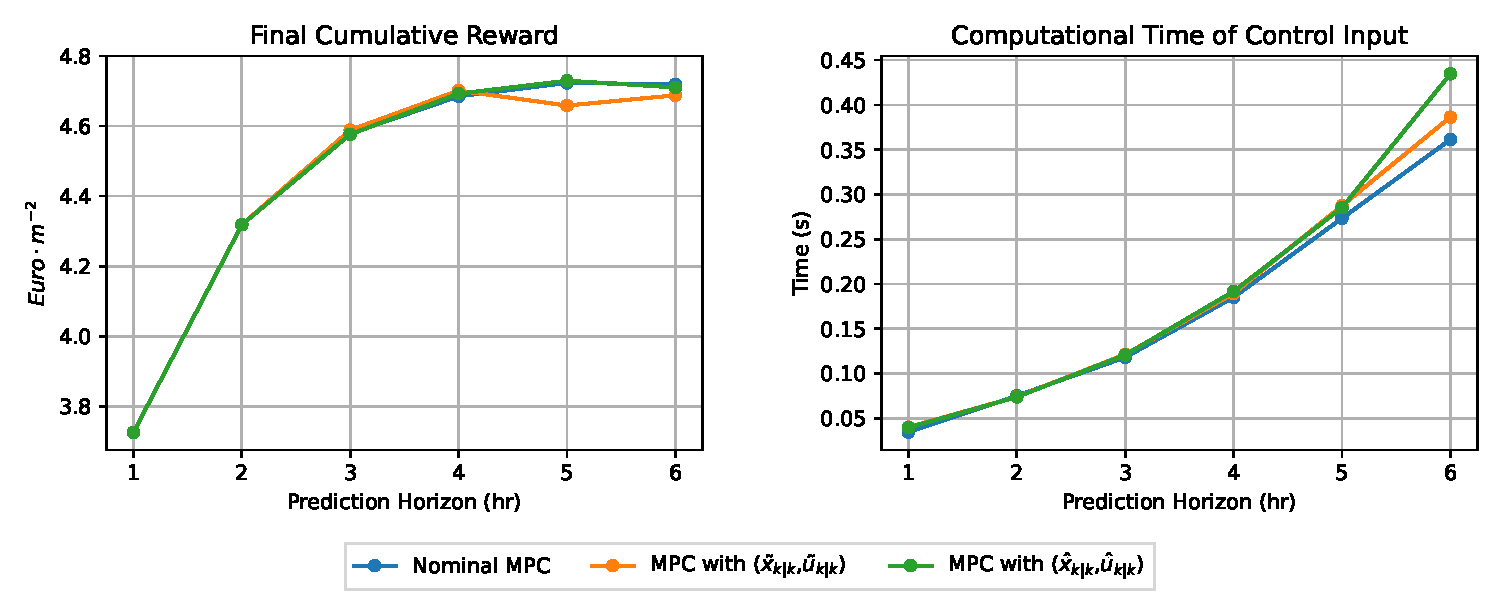
\includegraphics[width=\textwidth]{figures/rl_mpc_impl_1.eps}
	\caption{MPC vs MPC with initial guesses}
	\label{fig:rlmpc-impl1}
\end{figure}

\autoref{fig:rlmpc-impl1} presents the results of passing in initial guesses from the actor. Unrolling the actor from the current state and using the resulting state and control inputs as initial guesses (\autoref{eq:initial-guess-2}) seems to have very little impact on the final cumulative reward, however it noticeable increases the computational time of the control input. This could be because the initial guesses are derived from a less than optimal policy. Moreover, initial guesses by extending the prediction horizon from \autoref{eq:initial-guess-1} also has minimal impact on the final cumulative reward for shorter prediction horizons, and seems to be slightly beneficial for a 3 and 4 hour prediction horizon. However performance degrades significantly for a prediction horizon of 5 and 6 hours as compared to the nominal MPC. Additionally, computational also time increases. It would be expected that computational time decreases for both initial guesses. A reason for the sub-optimal performance may be due the initial guesses of the Lagrangian multipliers (the found Lagrangian multipliers from the previous solution). The actor's initial guesses may differ significantly from the previous solution, rendering the Lagrangian multipliers' guesses nonsensical. While the actor may offer initial guesses, they are insufficient for improving or assisting the MPC, and simply using the previous solution as an initial guess may be more beneficial. However, the importance of having optimal initial guesses becomes more significant as the prediction horizon is extended, as the problem complexity increases. Therefore, if a superior policy to the Nominal MPC were to provide initial guesses instead of a suboptimal policy at a longer prediction horizon, it could result in a more favourable outcome.

\section{Results - Implementations 2}

\begin{figure}[H]
	\centering
	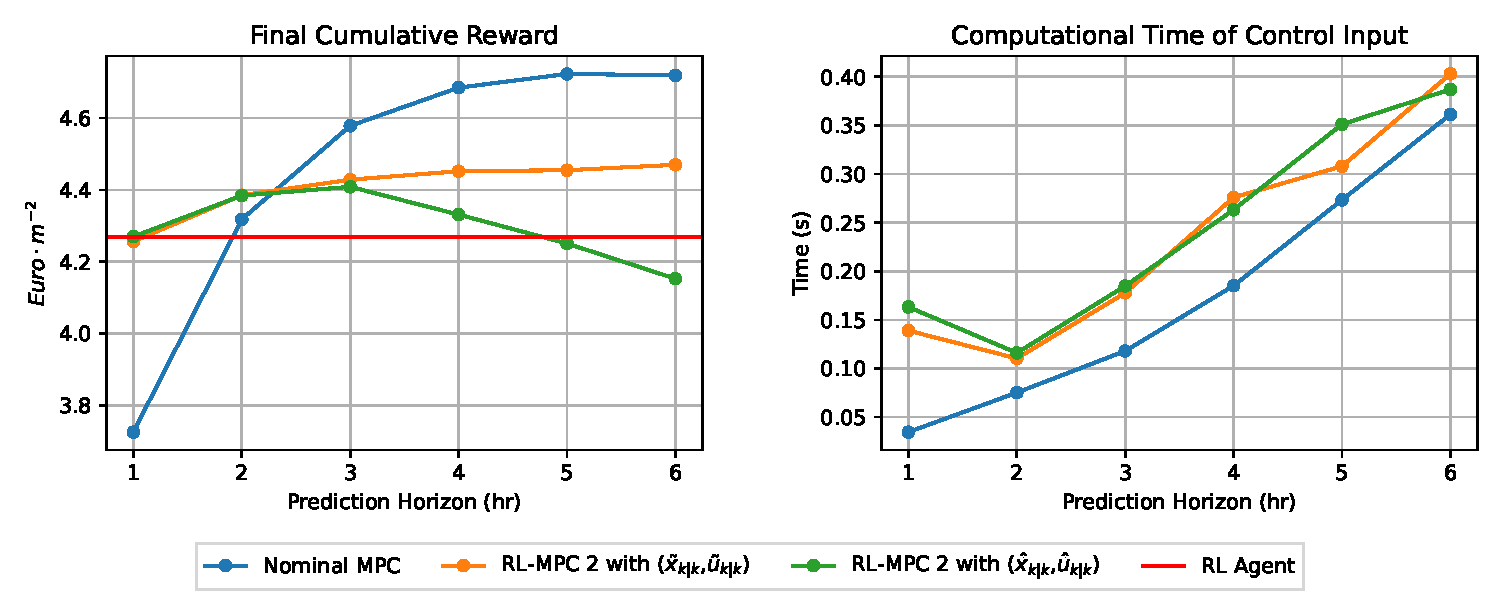
\includegraphics[width=\textwidth]{figures/rl_mpc_impl_2.eps}
	\caption{MPC with terminal constraints from agent}
	\label{fig:rlmpc-impl2}
\end{figure}

In order to guarantee that the RL-MPC policy achieves a performance level that is equal to or better than the RL policy, the approach described in Implementation 2 was used.  The performance of the resulting policies is illustrated in \autoref{fig:rlmpc-impl2}. It is evident that for a terminal constraint and initial guesses as given by \autoref{eq:initial-guess-1}, that the resulting policy is at least as good as the RL's, even at lower prediction horizons where RL performs better than MPC. Nevertheless, the RL-MPC policy exhibits notably inferior performance compared to the MPC policy when the prediction horizon exceeds 3 hours. Beyond the 3-hour mark, the MPC policy consistently outperforms the RL policy and RL-MPC policy.  While the implementation of RL-MPC may enhance the RL policy, it does not guarantee that the resulting policy will surpass the policy generated purely by MPC. If the RL policy is more competitive and surpasses the performance of the MPC, then implementing this RL-MPC implementation would be advantageous, as is the case for a prediction horizon of 1 and 2 hours. This marks a very important design choice. One can choose to either impose a terminal constraint to guarantee a certain level of performance or instead opt to extend the prediction horizon of the MPC. Again, by extending the horizon for the MPC controller is not guaranteed to perform better under economic optimization, therefore a safer choice may be to implement the terminal constraint as provided by the RL agent.
\\
The lack of performance guarantees for the terminal constraint and initial guesses, as indicated by equation \autoref{eq:initial-guess-2}, is evident in the decrease in performance, which is even worse than that of reinforcement learning, when longer prediction horizons are considered.\\

The computational time for the control input significantly increases when the prediction horizon is set to 5 or 6 hours. The terminal constraint may excessively limit the MPC due to the presence of a sub-optimal terminal constraint, particularly when dealing with longer prediction horizons.

\section{Results - Implementation 3}
This implementation aims to move away from the terminal constraint and allow the MPC more freedom by providing it with a terminal region constraint as outlined in \autoref{eq:terminal-region}, with a chosen $\delta = 5\%$, allowing for a $10\$$ deviation in the terminal state. As claimed in \cite{amritEconomicOptimizationUsing2011}, this could prove to be more beneficial than the terminal constraint, provided that an appropriate cost function is supplied. For this implementation, the cost function supplied is effectively $V(s) \equiv 0$. 


\begin{figure}[H]
	\centering
	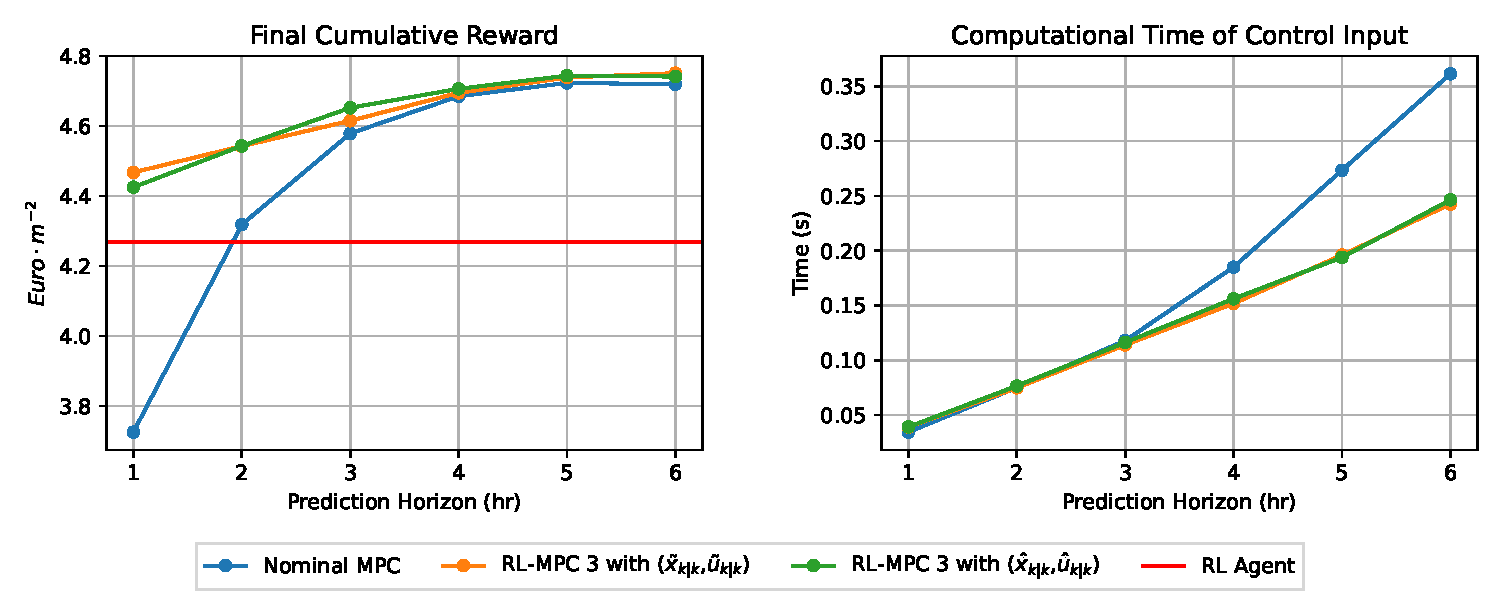
\includegraphics[width=\textwidth]{figures/rl_mpc_impl_3.eps}
	\caption{MPC with terminal region}
	\label{fig:rlmpc-impl3}
\end{figure}

The results from the implementation are depicted in \autoref{fig:rlmpc-impl3}. Shortening the prediction time horizons results in a substantial increase in the overall cumulative reward compared to both the standalone MPC and RL policies. Furthermore, the RL-MPC obtains a marginally superior final cumulative reward in comparison to the MPC even at longer prediction horizons. Lastly, it appears that this performance is increasing monotonically with an increase in prediction horizon, unlike for MPC. This could indicate that an appropriate cost function and terminal region has been found to  guarantee performance and stability. However, longer prediction horizons would be required to provide conclusive evidence of this.\\

Additionally, this terminal region also allowed for a lower computation time of the control inputs, with a more noticeable faster compute time at longer prediction horizons. This is likely because the terminal region is less limiting than the terminal constraint,  while also providing guidance to the MPC, resulting in reduced computational times.

It is noted that the resulting performance (increase in total cumulative reward and decrease in computational time) of the RL-MPC policy outperforms both standalone policies, even when the terminal region and initial guesses are supplied by a policy that performs substantially worse than the MPC controller. This underscores the necessity of giving certain future-oriented information to the EMPC in order to attain optimal economic advantage, performance, and stability. 

\section{Results - Implementation 4}
This implementation investigates the effect of a supplying the MPC with a cost function, specifically an approximate value function represented by a neural network.


\begin{figure}[H]
	\centering
	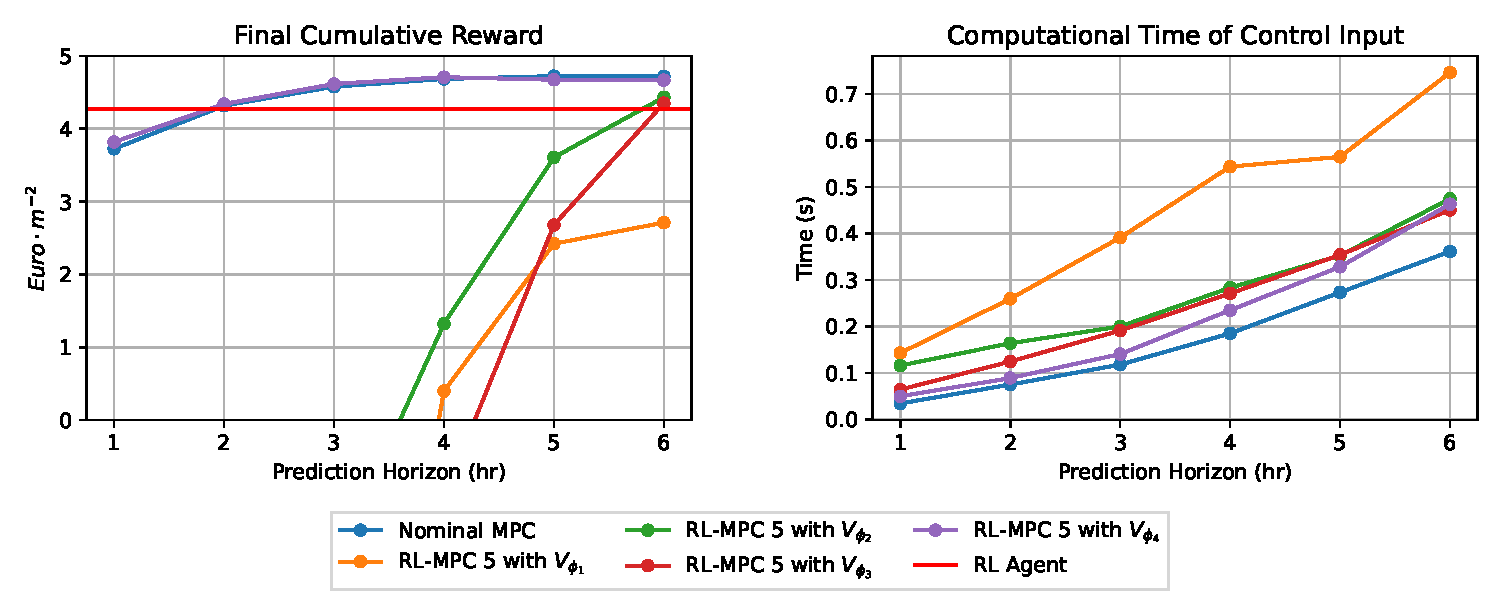
\includegraphics[width=\textwidth]{figures/rl_mpc_impl_4.eps}
	\caption{MPC with terminal cost function}
	\label{fig:rlmpc-impl4-all-states}
\end{figure}
\autoref{fig:rlmpc-impl4-all-states} is a naive implementation of merging RL and MPC. However, the outcomes are unsatisfactory in terms of both the overall cumulative reward and the computational time required for generating control inputs. Caution must be exercised when employing a neural network in an optimizer, as they possess a profoundly non-linear nature. As illustrated in \autoref{fig:rlmpc-impl4-all-states}, the performance deteriorates as the neural network becomes more intricate. The neural networks exhibit highly non-convex behaviour that may cause the MPC optimizer to become easily trapped in local optima. The only value function that seems to not destabilize the optimizer is $\tilde{V}_4$ which is also the only value function that exhibits a smooth behaviour, see \cref{rem:vf-smoothness}. The MPC's optimisation task is solely focused on maximising the drymass in this particular value function, with time being a constant parameter. However, for the other value functions, the MPC needs to optimise across all possible model states and inputs.Although this leads to more accurate inference for the value of the specific environmental state, it also introduces additional dimensions and consequently a greater number of possibilities for becoming stuck in local optima that may not be meaningful.\\
It is natural to observe an increase in computational time in \autoref{fig:rlmpc-impl4-all-states}. Once again, the extremely non-convex nature of the behaviour can disrupt the MPC optimizer and lead to unpredictable computational times. However, it is worth noting that $\tilde{V}_4$ consistently exhibits a predictable computational time, highlighting the significance of obtaining a high-quality value function.

\begin{figure}[H]
	\centering
	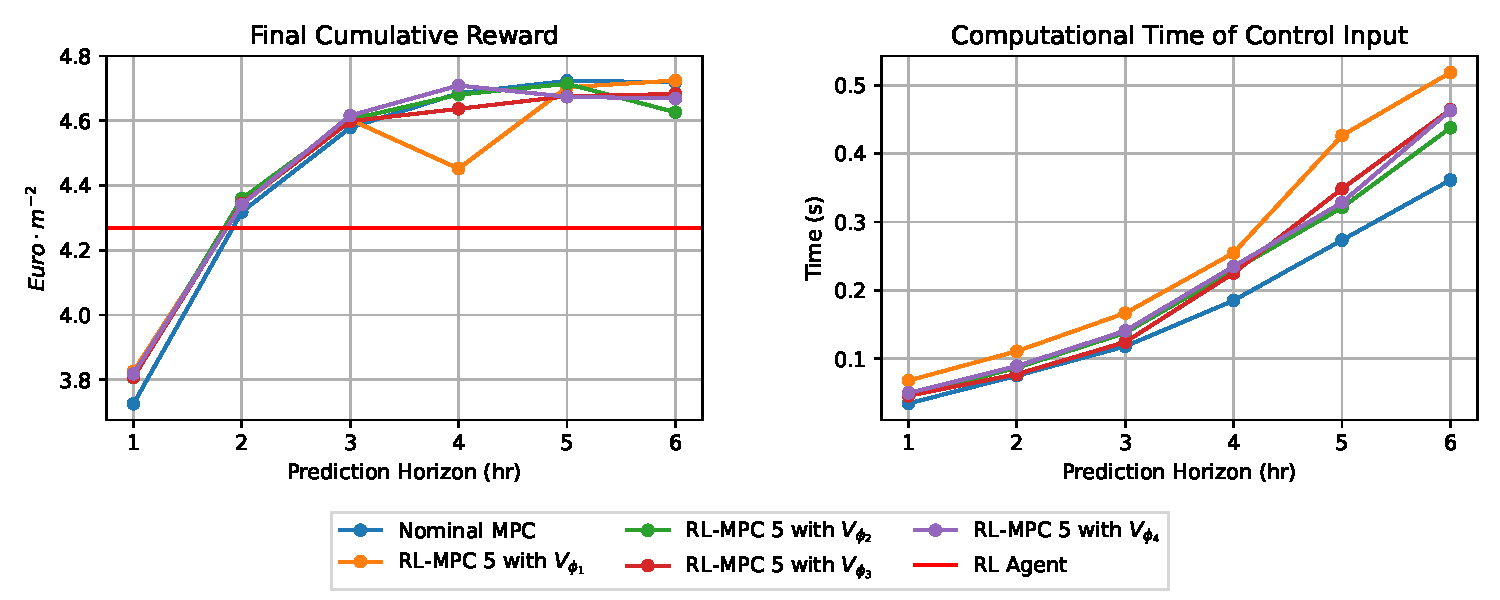
\includegraphics[width=\textwidth]{figures/rl_mpc_impl_4_1.eps}
	\caption{MPC with terminal cost function}
	\label{fig:rlmpc-impl4-only-drymass}
\end{figure}
To minimise the non-linearity of the value functions, the decision variables, except for the drymass, were kept fixed at their initial guesses. This was done because it is evident that the value of a state can be estimated based solely on the current time and the state of the drymass.Thus, the optimisation process was exclusively focused on optimising the dry mass, as was  done with $\tilde{V}_4$. The performance of the resulting RL-MPC policy is demonstrated in \autoref{fig:rlmpc-impl4-only-drymass}. The addition of the value functions improves the final cumulative reward over MPC at shorter prediction horizons but degrades performance for longer prediction horizons (5 and 6hr). Although the value functions have been simplified, increasing the prediction horizon allows the MPC's optimization process to get trapped in local optima, this could be the reason for the observed performance degradation in \autoref{fig:rlmpc-impl4-only-drymass}. Moreover, the simplification of the value function also resulted in more consistent times, with very little increase as compared to the nominal MPC.\\

$\tilde{V}_4$ was used for further testing, since it exhibits the greatest performance increase (final cumulative reward) over the nominal MPC (1-4hrs) as compared to the other simplified value functions. The performance of $\tilde{V}_4$ is expected to be superior to the others because it was trained exclusively on the drymass state and time, enabling it to make more accurate predictions of the value of a specific state using only these two inputs. These results suggests that a value function can increase performance over nominal MPC, but necessarily over the Rl policy that it was derived from. In addition, in order for the value function to be effective, it should have a minimal number of local optima while maintaining accuracy. Furthermore, it should be smooth and capable of generalising effectively across the state space to ensure reliable performance. Lastly, it is important to balance the performance gains with the increased computational time, and as shown in \autoref{tab:rl-mpc-v4}, the increase in computational time, far outweighs the marginal performance increase for shorter prediction horizons.

\begin{table}[H]
	\centering
	\begin{tabular}{|c|cccccc|}
		\hline
		&1hr&2hr&3hr&4hr&5hr&6hr\\
		\hline
		Final Cumulative Reward Increase(\%) &2.484 &0.525&0.814&0.512&-1.041& -1.069\\
		\hline
		Computational Time Increase     (\%) &50.888 &40.358&30.859&29.062&14.243& 23.013\\
		\hline
	\end{tabular}
	\caption{RL-MPC $\tilde{V}_4$ performance comparison compared to MPC}
	\label{tab:rl-mpc-v4}
\end{table}



\section{Results - Implementation 5 and 6}
Implementation 5 aims to incorporate both a terminal region constraint as well as a terminal cost function. $\tilde{V}_4$ is used as a cost function with a terminal region generated by initial guesses as in \autoref{eq:initial-guess-1}, with a $\delta_T =5\%$. Implementation 6 solves two problems, each with its own initial guesses and terminal region (\autoref{eq:initial-guess-1} and \autoref{eq:initial-guess-2} respectively).It determines the optimal policy by evaluating the terminal state in each solution using the value function.
\begin{figure}[H]
	\centering
	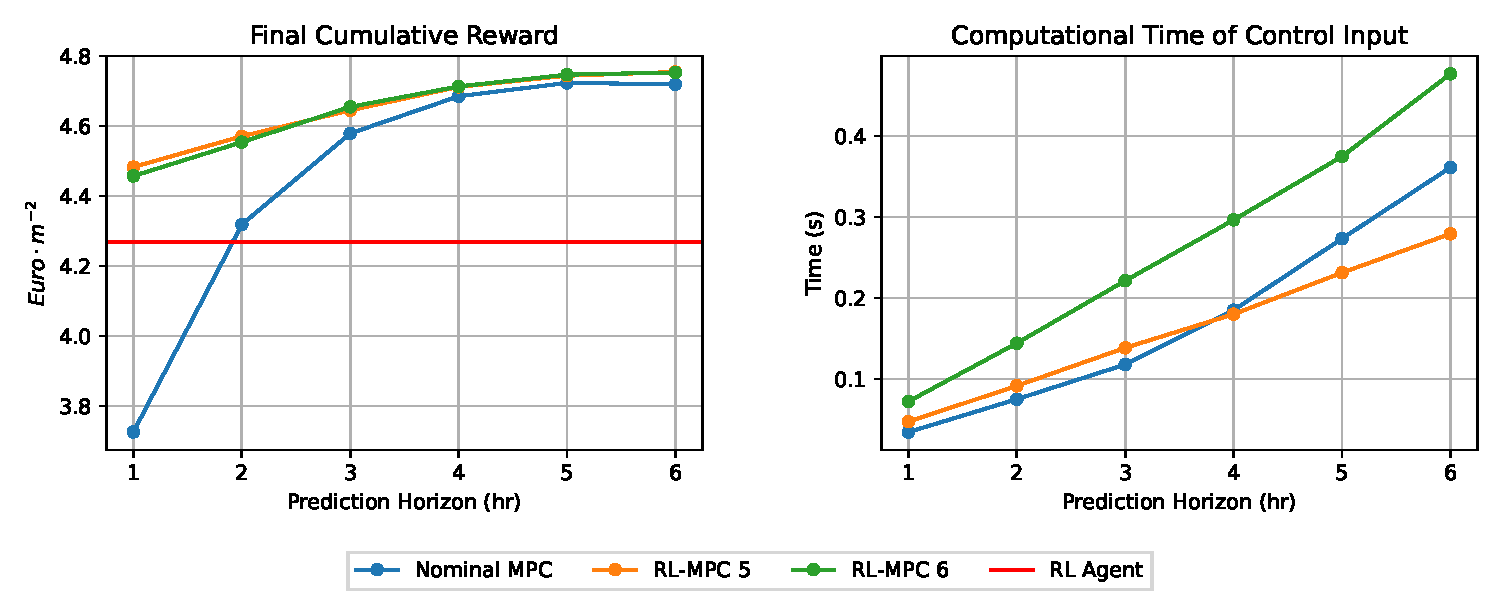
\includegraphics[width=\textwidth]{figures/rl_mpc_impl_5_6.eps}
	\caption{MPC vs RL-MPC with terminal region and cost function vs RL-MPC solving two separate problems and evaluating best policy with value function}
	\label{fig:rlmpc-impl5-6}
\end{figure}
As demonstrated in \autoref{fig:rlmpc-impl5-6}, both implementations outperform the standalone MPC and RL policies across all MPC prediction horizons. The computational time of implementation 6 is notably higher because it solves two optimisation problems instead of just one. Nevertheless, it is possible to solve the 2 problems in parallel, effectively reducing the computational time by half. Although the performance gains are substantial as compared to the standalone MPC, it is noted that majority of this performance increase is due to the terminal region constraint. In addition, this constraint on the terminal region also seems to make the performance increase monotonically, even with the addition of the value function. Furthermore, despite the inclusion of a neural network in the optimisation problem (Implementation 5), the computational time is reduced to a similar level as the standalone MPC when a terminal region constraint is present. 


However , whether a value function is necessary when the terminal region
\section{Final Result and Conclusion} \label{section:final-rl-mpc-nominal}
The three best implementations are compared, namely Implementation 3 (with guesses and terminal region provided by \autoref{eq:initial-guess-1}), Implementation 5 and 6.
\begin{figure}[H]
	\centering
	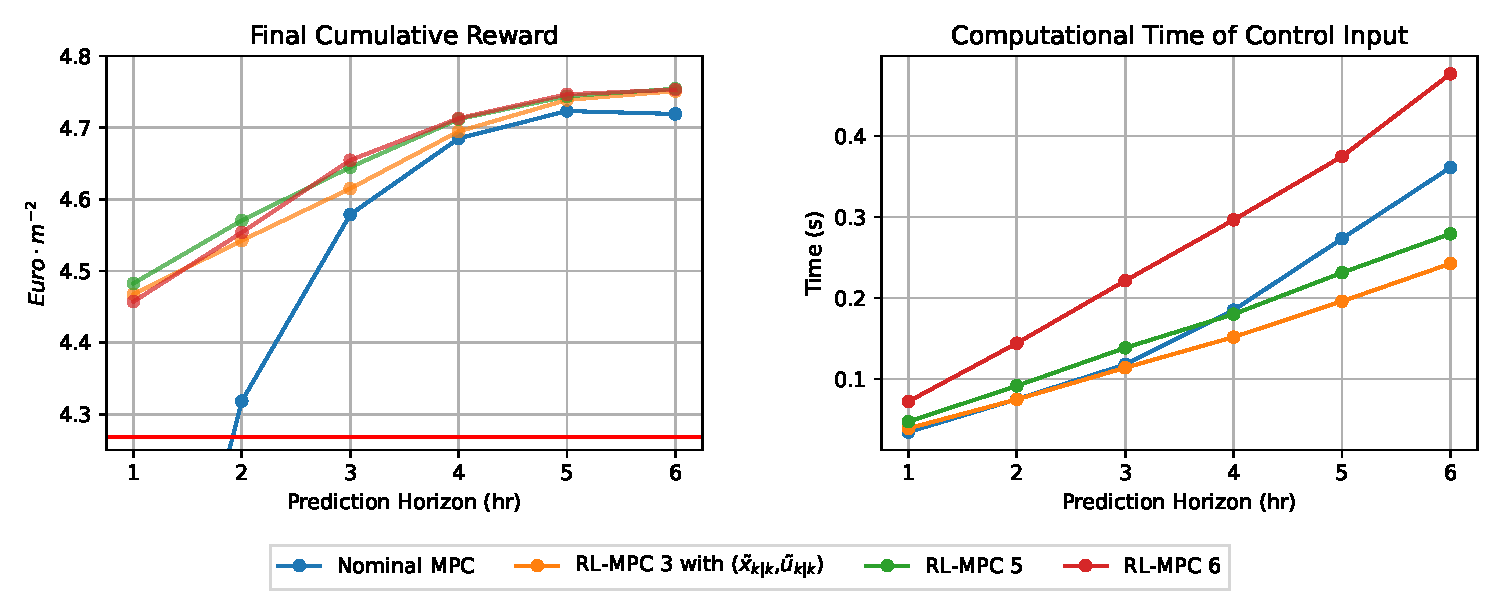
\includegraphics[width=\textwidth]{figures/rl_mpc_impl_final.eps}
	\caption{MPC final }
	\label{fig:rlmpc-final}
\end{figure}

The final results of the mentioned implementations are shown in \autoref{fig:rlmpc-final}. While the inclusion of a terminal region is the primary factor in improving performance, the incorporation of the value function can additionally enhance performance, albeit with the drawback of increased computational time. This suggests that the value function and terminal region provided by Rl satisfy the necessary assumptions to ensure performance of an EMPC. However, a formal proof would be needed to confirm this conclusively. Moreover, the increase in computational time is not that drastic when a neural network is implemented, especially with the addition of a terminal region to aid the MPC in finding solutions faster. While the computational time increase may appear insignificant, this system is relatively uncomplicated compared to others. If this approach is used in highly complex systems, this increase in computational time could result in destabilizing the system. Therefore any methods in reducing the computational time is highly beneficial. Moreover, it seems that there is very little benefit to adding a cost function when the advantages of adding a terminal constraint is already so beneficial.


\begin{table}[H]
	\centering
	\caption{RL-MPC 3 and 5 vs MPC and RL}
	\label{tab:rlmpc-3-5-vs-MPC-and-RL}
	\resizebox{\columnwidth}{!}{%
		\begin{tabular}{|c|cc|cc|cc|cc|cc|cc|cl|}
			\hline
			& \multicolumn{2}{c|}{1hr} & \multicolumn{2}{c|}{2hr} & \multicolumn{2}{c|}{3 hr} & \multicolumn{2}{c|}{4 hr} & \multicolumn{2}{c|}{5 hr} & \multicolumn{2}{c|}{6 hr} & \multicolumn{2}{c|}{RL  @ 1 hr} \\
			& Perf & Time & Perf & Time & Perf & Time & Perf & Time & Perf & Time & Perf & Time & \multicolumn{2}{c|}{Perf} \\ \cline{2-15} 
			RL-MPC 3 (\%) & 19.91 & 10.91 & 5.191 & 2.38 & 0.79 & -5.38 & 0.21 & -8.47 & 0.328 & -16.2 & 0.67 & -18.95 & \multicolumn{2}{c|}{4.67} \\
			RL-MPC 5 (\%) & 20.32 & 24.26 & 5.84 & 18.26 & 1.44 & 44.37 & 0.57 & 3.68 & 0.435 & 2.71 & 0.746 & -7.86 & \multicolumn{2}{c|}{5.02} \\ \hline
		\end{tabular}%
	}
\end{table}

\autoref{tab:rlmpc-3-5-vs-MPC-and-RL} displays the performance increase of RL-MPC 3 and RL-MPC 5 against the nominal MPC and a comparison with RL at a 1hr prediction horizon. Incorporating both a terminal region and value function  appears to offer minimal advantages compared to only using a terminal region, as the marginal improvement in performance results in a significantly larger increase in computational time. This reiterates the importance of reducing the computational cost of the neural network in the optimization problem. As seen in \autoref{fig:rlmpc-final}, RL-MPC 6 offers promising results as an alternative method to using the value function, and could yield even more benefits when more than two initial trajectories and terminal regions are provided by various agents and methods. The computational time of RL-MPC 6 can be theoretically halved by solving the problems in parallel, resulting in a compute cost similar to RL-MPC 3 and a similar performance to RL-MPC 5. Further research should be conducted on this implementation in the future.\\
While the combination of RL and MPC shows promising results, it is important to note that the simulations remain deterministic. These results primarily indicate which implementations are worth testing further in a stochastic environment, to create a more accurate depiction of reality. Moreover, is may be tempting to use RL-MPC 2 (with terminal constraint) to guarantee performance as good as RL. However, in a stochastic environment, this may not be practically achievable and there are no equivalent performance guarantees available. It may not be feasible because the terminal constraint, as determined by the generated reference trajectory, may not be attainable due to the random nature of the state evolution. Consequently, allowing a terminal region relaxes this constraint and makes the problem computational tractable. Finally, a value function derived from a policy that inherently considers uncertainty can provide the MPC with valuable insights regarding the impact of uncertainty on its calculated control actions. Therefore, RL-MPC 3 and RL-MPC 5 are suitable choices for testing in a stochastic environment.



